\documentclass[fleqn,10pt]{wlscirep}

\usepackage[acronym,style=alttree, toc=true, shortcuts, xindy, nomain, nonumberlist]{glossaries}
\usepackage[utf8]{inputenc}
\usepackage[T1]{fontenc}
\usepackage{textcomp}
\usepackage{bm}
\usepackage{siunitx}
\usepackage{amsmath}
\usepackage{nccmath}
\usepackage{indentfirst}
\usepackage{multirow}
\usepackage[version=3]{mhchem}
\usepackage{csquotes}
\usepackage{biblatex}
\addbibresource{sample.bib}



\setcounter{secnumdepth}{4}



\newcounter{subsubsubsection}[subsubsection]
\def\subsubsubsectionmark#1{}
\def\thesubsubsubsection {\thesubsubsection 
	.\arabic{subsubsubsection}}
\def\subsubsubsection{\@startsection
	{subsubsubsection}{4}{\z@} {-3.25ex plus -1
		ex minus -.2ex}{1.5ex plus .2ex}{\normalsize\bf}}
\def\l@subsubsubsection{\@dottedtocline{4}{4.8em}
	{4.2em}}


\DeclareSIUnit{\Bit}{~Bit}




%%%%%%%%%%%%%%%%%%%%%
% ACRONYMS/GLOSSARY	%
%%%%%%%%%%%%%%%%%%%%%

\newacronym{ppv}{PPV}{Positive Predictive Value}
\newacronym{mcs}{MCS}{Monte Carlo simulation}
\newacronym{LOD}{LOD}{Limit of Detection}

\glssetwidest{THISWIDE} % adjust length as needed
\makeglossaries
\makeindex

\begin{document}
	
	\title{Improving Pooling-Strategies for Increasing the Test Capacity and Reliability of RT-qPCR of Samples out of Populations with low Prevalence} 
	
	
	%improve order of authors maybe use a circle (it's a really old list.)
	\author[*]{Kuo-Yi Chao}
	\author[*]{Leonhard Kuboschek}
	\author[*]{Leo T. Peters}
	\author[*]{Christoph Schierholt}
	\author[*]{PranavKumar Shadamarshan}
	
	%\affil[1]{Affiliation, Department, City, Country}
	%\affil[2]{Affiliation, Department, City, Country}
	
	\affil[*]{All authors have contributed equally to this report, the names are sorted alphabetically by last name}
	
	
	\begin{abstract}
		
		SARS-COV-2 has spread through the world and wreaked havoc to unforeseen levels. The lack of information about the virus has specifically made it difficult, while in the pursuit it has baffled medical experts due to the lack of readily available testing kits. RT-qPCR stands as the golden standard procedure for diagnosis of COVID-19. Here, we propose a strategy to increase the testing capability by pooling multiple samples. It is a pure strategic manipulation by mixing samples with the aim of obtaining maximum possible information, with a given amount of resources.
		In this report we present a way to evaluate the efficiency of a test by applying concepts from information theory. By evaluating the efficiency and considering statistical values, that describe the quality of the test results, it is possible to come up with pooling strategies, that can be parametrized to suit the desired requirements. A pooling strategy is an algorithmic description of how to pool different samples together and of how to proceed after any possible test results.
		
		In this report we come up with multiple pooling strategies and evaluate their performance at different prevalence. We use Monte Carlo Simulation to recreate test situations and to statistically describe the sensitivity, specificity, the positive and negative predictive values and the test efficiency.
		Our simulation model relies on two implementations, that statistically describe a PCR like diagnostic test and our suggested test strategies.
		
		We were able to show, that we can theoretically improve the number of tested persons by at least an order of magnitude at low prevalence while sustaining a high level of sensitivity.
		At the same time our suggested strategy resolves the issue of a poor positive predictive value at lower prevalences, as it scales with the prevalence.
		
		
		
	\end{abstract}
	
	\flushbottom
	
	
	\maketitle
	
	\thispagestyle{empty}
	
	\tableofcontents 
	
	\section{Introduction}
	
	SARS-COV-2 (Severe acute respiratory syndrome coronavirus 2) or 2019-nCOV is a type of bat-borne virus that causes respiratory illness. It is the mutational successor to SARS-COV-1 which was identified in the 2003 outbreak largely in Asia. They are a class of RNA viruses that causes coronavirus disease 2019 (covid-19). With no immunity in the community and asymptomatic transmissions, covid-19 has been announced a pandemic and a matter of public health emergency. Covid-19 has been taking over the world like a wildfire and the economies of countries have succumbed to it. The main reason for this letdown is unavailability of ample testing kits due to inefficient testing.\\
	
	With faster and efficient testing strategy, a country knows where it stands amidst this pandemic. For instance, South Korea in the first week of its critical period had already conducted 300,000 tests, establishing 600 test centres across the country. It had halved the number of infections in just a week [1]. On the other end of the spectrum, Italy and the US has/is failing to cope up with the pandemic. So much so that Italy could not keep up with the pandemic because they did not know where they stood in the curve because of the inefficiency in testing samples. Efficient testing could give more information on the current situation in the pandemic and allow governments to take more appropriate measures. At a large scale, it could reward the community by flattening the curve faster and decreasing the R0. Randomized community testing could also be made possible which is highly advantageous to isolate asymptomatic infected people disrupting the infection chain. The delay in testing has and is still costing lives [1-3]. The take home message from these scenarios is that high capacity testing provides more information upon which a country could take a standpoint and act in preparedness. We require a method to increase the efficiency of testing without excess resources, or labour. So, we propose a strategy for efficient testing of SARS-COV-2 by sample pooling.
	
	
	\section{Methods}
	
	\subsection{Information Theory}
	A measure for the amount of information is the so called \glqq entropy\grqq{} and is associated with the unit \si{\Bit}. It forms the basis of information theory, which was initially developed by Shannon \cite{Shannon} and is mainly used in communication engineering. In this paper we will apply it to pool testing in order to estimate the potential of an optimal pooling strategy and to compare the developed strategies to such optimal performance.\\
	
	The relevance of information theory in the context of large scale testing can be understood as follows: The total amount of information on the patients state of a population is bounded, as we are looking at a finite number of people with a binary state (infected or not infected). By applying pool testing, the information obtained by a test can be increased, which allows us to require less tests in order to evaluate the peoples state.\\
	
	The amount of information carried by a Bernoulli distributed (or binary) random variable can be closely related to the information carried by a diagnostic test, which also yields a binary result (positive or negative).\\
	
	Information theory tells us, that the entropy of such random variable is maximized, if its both outcomes are equally distributed. In this case the amount of information is \SI{1}{\Bit}. This is also the maximum information obtained by a single diagnostic test that does not allow any errors in result.\\
	
	In the case of single testing with ideal tests the amount of information obtained by one test is equal to the amount of information carried by one patients state. This is why we need exactly one test per person if we conduct single testing. The entropy of the populations state depends on the prevalence and can be estimated by regarding each patient as a binary random variable with probability equalling to the prevalence $p_{inf}$:\\
	
	\begin{ceqn}
		\begin{equation}
		H(p_{inf}) = \left[-p_{inf} \cdot \log_2(p_{inf})-(1-p_{inf}) \cdot \log_2(p_{inf})\right] \si{\Bit}
		\end{equation}
	\end{ceqn}
	
	\begin{figure}[ht]
		\centering
		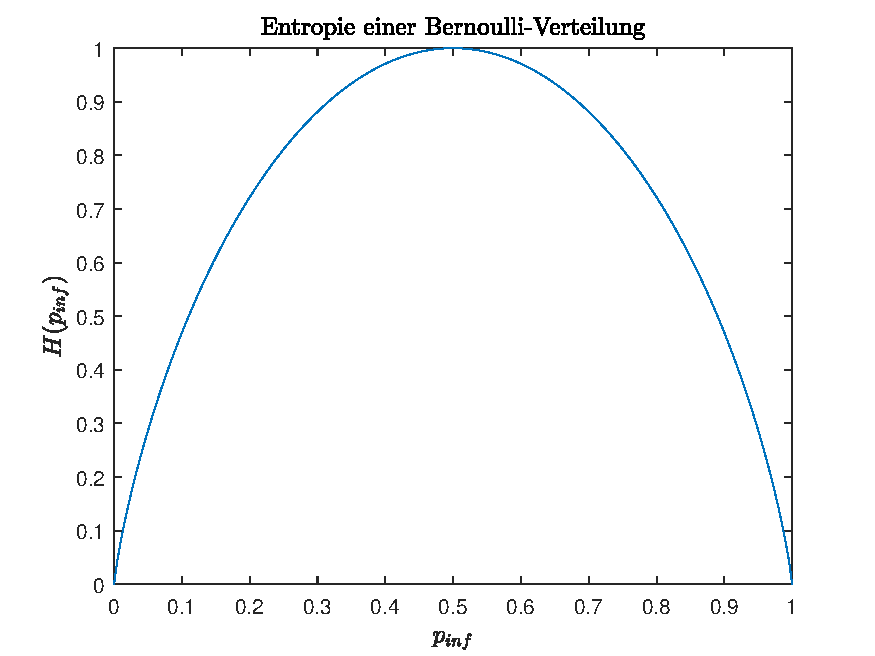
\includegraphics[width=0.6\textwidth]{pics/Bin_Entropie.pdf}
		\caption{Amount of Information obtained by a single and ideal test vs. prevalence $p_{inf}$}
		\label{fig:bin_entropie}
	\end{figure}
	
	Fig. \ref{fig:bin_entropie} shows a maximum in entropy of a test, if its outcome is equally distributed. It is interesting to note, that the entropy only varies slightly for small deviations from the optimum, while it drops to zero, when the prevalence is $0$. This means that single testing cannot be used efficiently at low prevalences. Prevalences above $0.5$ will not be regarded in this work.\\
	
	This means that single testing cannot be used efficiently at low prevalences. Prevalences above 0.5 will not be regarded in this work. By pooling samples together, we end up with a mix. We can increase the probability of such a mix containing at least one positive sample by adding more samples. For low prevalence this leads to a higher amount of information obtained by one test performed on this mix, when comparing it to single testing.
	This will be further carried out in section \ref{sec:analytics}.
	
	
	Another important measure from information theory is mutual information. It indicates how much information of one random distribution can be obtained by another random distribution. If a diagnostic test was never leading to an error, the distribution of a persons state and of the test result a closely coupled, which results in the mutual information being equal to the entropy of the person's state. If however errors occur, the information lost during the conduction of a test (through false negatives and false positives) is the difference between the information of the person's state and the mutual information, which is depicted in fig. \ref{fig:mutual_information}. In the case of an imperfect diagnostic test, it can be useful to maximize the mutual information between the population's state and the test results instead of maximizing the entropy.\\
	
	\begin{figure}[ht]
		\centering
		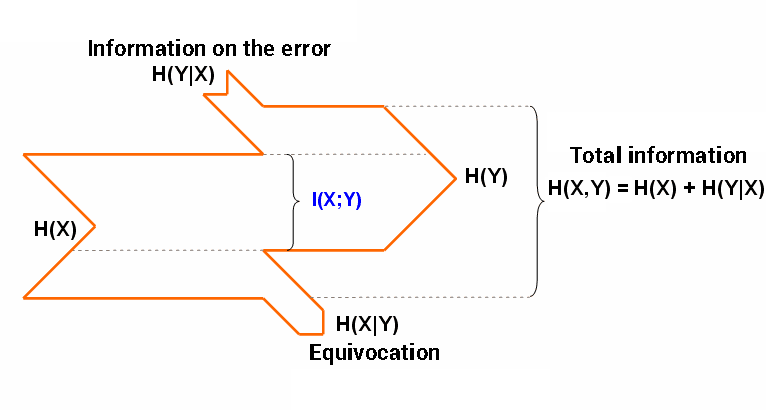
\includegraphics[width=0.7\linewidth]{pics/Entroy_XY_Eng.png}
		\caption{Mutual information \cite{Transinformation} of the patients state X and the test result Y.}
		\label{fig:mutual_information}
	\end{figure}
	
	Another use for the mutual information is the evaluation of conducting multiple diagnostic tests on subsets of a bigger pool of samples. Just as it is desirable to increase the mutual information between the population's state and the test results, it is also desirable to decrease the mutual information between the test results of multiple tests. This originates in the idea, that obtaining the same information by multiple tests will not increase the overall information retrieved. The concept of mutual information will only be used as an instrument to emphasize differences between strategies, while it will not be used for optimization as part of this work.
	
	
	\subsection{RT-qPCR}
	Detection of the viral infection in patient samples is performed by Reverse transcription- quantitative polymerase chain reaction (RT-qPCR) analysis. It works by selectively amplifying the viral RNA gene and by detecting the amplified viral gene. It is the most common analytical technique used to analyze SARS-COV-2 in the current pandemic situation. RT-qPCR could be done in a single step or a longer double step method. WHO recommends either of these types. From publications surfacing around the world, the common trend is a one-step RT-qPCR.\\
	
	The analytical technique only works on DNA. So, it is imperative to convert the viral RNA to DNA in order to be detected. The first protocol is to convert the existing RNA to DNA (Reverse Transcription). Followed by the amplification and detection of the DNA samples (quantitative PCR). The amplification and detection takes place in several cycles of the analysis. Each cycle takes \SI{45}{seconds}. 45 such cycles are performed and a readout is taken at the end of each cycle. Under the presence of the viral gene the readout value increases with every cycle and surpassess the threshold (above noise levels), but under the absence of any infection the readout stays below the threshold in all cycles. For the sake of error corrections, any readout that surpassess the threshold in late cycles might be considered false positive.\\
	
	WHO recommends a three assay workflow, first line screening, confirmatory and discriminatory assays. First line assay confirms the presence of E gene, which would confirm the presence of Bat related viruses in the sample. Confirmatory assay (RdRp assay I) proclaims the presence of SARS related viruses. Finally discriminatory assay (RdRp assay II) provides the verdict for the novel SARS-COV-2 infection in the sample. One assay succeeding the other only in the case of a positive result.\\
	
	A typical commercial RT-qPCR reagent consists of a 2x reaction mixture, BSA (Bovine Serum Albumin) to increase efficiency, Primers for amplification of selective genes and probes for the detection of selective genes. The design of primers and probes play a major role in the RT-qPCR analysis. A probe is a small nucleotide stretch (TaqMan probe) that attaches to the said viral gene and fluoresces upon each amplification cycle. This fluorescence is the readout at the end of each cycle. The primer and probe designs have been optimized and reported by WHO as follows:
	\begin{table}
		\begin{center}
			\begin{tabular}{ |c|l|l| } 
				\hline
				Assay & oligonucleotide ID/ use & sequence 5’ $\rightarrow$ 3’ \\ 
				\hline
				\multirow{3}{*}{E gene} & E Sarbeco F2 (Forward) & ACAGGTACGTTAATAGTTAATAGCGT \\  \cline{2-3}
				& E Sarbeco R2 (Reverse) & ATATTGCAGCAGTACGCACACA \\ \cline{2-3}
				& E Sarbeco P1 (probe for detection of E gene) & FAM-ACACTAGCCATCCTTACTGCGCTTCG-BBQ \\ \cline{2-3}
				\hline
				\multirow{4}{*}{RdRp gene} & RdRP SARSr-F2 (Forward) & GTGARATGGTCATGTGTGGCGG \\  \cline{2-3}
				& RdRP SARSr-R1 (Reverse) & CARATGTTAAASACACTATTAGCATA \\ \cline{2-3}
				& RdRP SARSr-P2 (detects only SARS-COV-2) & FAM-CAGGTGGAACCTCATCAGGAGATGC-BBQ \\ \cline{2-3}
				& RdRP SARSr-P1 (detects all bat related SARS-CoVs) & FAM-CCAGGTGGWACRTCATCMGGTGATGC-BBQ \\
				\cline{1-3}
				
				
				
			\end{tabular}
			\caption{Primers and Probes}
			\label{tab:primes}
		\end{center}
	\end{table}
	
	The reaction mixture has \SI{25}{\micro\litre} - \SI{5}{\micro\litre} of RNA, \SI{12.5}{\micro\litre} of 2x reaction buffer (made for one-step RT-qPCR with Platinum Taq Polymerase) \SI{1}{\micro\litre} of reverse transcriptase, \SI{0.4}{\micro\litre} of 50 mM \ce{MgSO4}, \SI{1}{\micro\litre} of required primers, \SI{0.5}{\micro\litre} of required probes and made up for the rest of the volume with sterile RNase free water to make \SI{25}{\micro\litre}. Thermal cycling is performed at \SI{55}{\degree\celsius} for 10 min for reverse transcription, followed by \SI{95}{\degree\celsius} for \SI{3}{\minute} and then 45 cycles of \SI{95}{\degree\celsius} for \SI{15}{\second}, \SI{58}{\degree\celsius} for \SI{30}{\second}.
	
	
	\subsection{Assumptions}
	
	In order to examine the effect of our pooling strategies, we implemented two models of the PCR (PCR simple and PCR dilution dependent) with varying degrees of realism. Another assumption addresses the distribution of viral loads within the patients.
	
	\subsubsection{PCR simple}
	\label{sec:PCR_simple}
	PCR is a highly sensitive and specific technique. Hence, a tiny mishandling or variation would go a long way in the end result. The number of reagents added at very small amounts call for critical experimental handling. Other issues lie in the handling, transportation and storage of the clinical samples. With proper experienced manpower sensitivity is pointed to $98 \%$ and specificity at $99 \%$. The modelling in this case does not encompass the concentration, thermal cycles of qPCR run or other chemical parameters. Instead, the model considers whether any sample within a pool is positive. After applying the confusion matrix (based on the sensitivity and specificity), the output is generated accordingly. A limitation of this model is that it does not reflect the dilution of samples in pools, which will overrate the performance of sample pooling. On the other hand, the correlation of concentration between pools is not being considered, which will underrate its performance.
	
	
	\subsubsection{PCR dilution dependent}
	\label{sec:PCR_dilution_dependent}
	PCR is a quantitative technique and the results are highly affected by the initial viral gene content. The concentration of viral genes in a sample is denoted by copies/ml. A qPCR analysis requires a sample with a minimum content of viral copies/ml in order to detect it. This is known as the \gls{LOD}. It is important to know the \gls{LOD} of the E genes and the RdRp genes, as sample pooling will effectively lower the copies of the viral gene in the samples. The \gls{LOD} for E gene is found to be 6.65 $\pm$ 2.95 copies/reaction and for RdRP 5.15 $\pm$ 2.45 copies/reaction.\\
	
	\begin{figure}[ht]
		\centering
		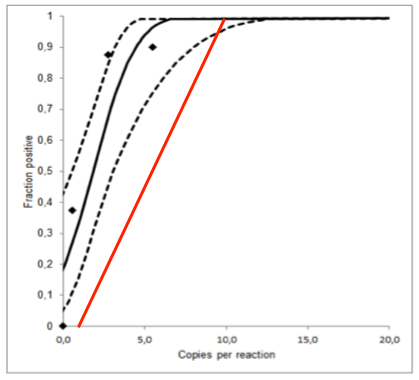
\includegraphics[width=0.6\textwidth]{pics/LOD_1-10.png}
		\caption{Limit of Detection \cite{WHO_Report} with our model (red)}
		\label{fig:LOD}
	\end{figure}
	
	For our model we use linear interpolation between 4 copies/reaction (\SI{0}{\percent}) and 10 copies/reaction (\SI{99.5}{\percent}) to determine the sensitivity. It remains at \SI{99}{\percent} for concentrations above 10 copies/ml as depicted in fig. \ref{fig:LOD}. The specificity is not modelled concentration dependent and is set to \SI{99}{\percent}. 
	
	
	\subsubsection{Viral Load}
	The severity of the viral infection is characterized by its number of RNA copies in the patient sample. Clinical samples have shown around 1.6 x 106 RNA copies/ml [5]. The minimum amount required to analyse the sample is 400 RNA copies/ml [6].\\
	
	This would technically mean that we could dilute a sample 4000 times and still be able to detect it. Pooling multiple samples would dilute the samples, but within a certain range would still be detectable. A test concluded that an interpretable signal was obtainable by pooling 32 samples together [7]. In our model we generate a discrete viral load distribution $c_{vir}$, which we chose by inspection. For effects introduced by the dilution we assume a binomial distribution of the resulting virus concentration, as we are dealing with discrete particles on such a low scale. \\
	
	We assume that \SI{1}{\milli\liter} with $n_{vir} = c_{vir} \cdot \SI{1}{\milli\liter}$ RNA copies is being taken from each patient (where this number does not affect the outcome too much - it simply has to be chosen sufficiently big). From that volume $\frac{\SI{5}{\micro\liter}}{n_{pool}}$ where $n_{pool}$ denotes the number of samples per pool is being mixed. The model from the binomial distribution results from the thought, that each virus particle within that \SI{1}{\milli\liter} is equally distributed and therefore within the final mix with a probability $p_{in pool} = \frac{\SI{5}{\micro\liter}}{n_{pool} \cdot \SI{1}{\milli\liter}} = \frac{1}{200 \cdot n_{pool}}$. As $n_{vir} \geq 50$ and $p_{in pool} \leq 0.05$ it is safe to use the poisson-approximation \cite{poisson_approx}, which can be calculated faster in our simulation.
	
	
	
	%let us insert the distribution of viral load as a histogram or table here.
	
	\subsection{Strategy Evaluation Measure}
	Common measures for evaluating the quality or correctness of a test are the sensitivity and the specificity.
	\begin{itemize}
		\item $Sensitivity = \frac{TP}{TP+FN}$ is the probability that the test conducted on an infected person turns positive. The reasons for the sensitivity to be suboptimal in the case of RT-qPCR for SARS-CoV-2 can be
		\begin{itemize}
			\item{low viral load of the patient}
			\item{poor extraction of the sample from the patient}
			\item {too little virus particles in the sample}
			\item {other handling errors}
		\end{itemize}
		\item $Specificity = \frac{TN}{TN+FP}$ is the probability that the test conducted on a non-infected person turns negative. The reasons for the specificity to be suboptimal in the case of RT-qPCR for SARS-CoV-2 can be
		\begin{itemize}
			\item Non specific binding of the XXX (very unlikely)
			\item contamination of the collected samples
			\item other handling errors
			
		\end{itemize}
	\end{itemize}
	Such effects have to be modelled accurately, as the evaluation of the testing strategies relies greatly on the scalability and correlation between these errors.\\
	
	Another measure for the quality of the generated test results are the predictive values:
	\begin{itemize}
		\item The positive predictive value  $PPV = \frac{TP}{TP+FP}$ describes the probability of a person with a positive test result actually being infected. This value is decreased by an increasing number of false positives.
		\item The negative predictive value  $NPV = \frac{TN}{TN+FN}$ describes the probability of a person with a negative test result actually being not infected. This value is decreased by an increasing number of false negatives.
	\end{itemize}
	It is important to note that the predictive values differ from the sensitivity and specificity in that they also consider the prevalence.\\
	
	A typical problem at very low prevalence arises from the fact that the number of false positives can exceed the number of true positives easily even for tests with a high specificity \cite{ppv_problem}. In practice, this reduces the usability of tests on large scales without considering symptoms or without considering high risk contacts.\\
	
	An important metric for evaluating the efficiency of the test strategies is the average number of tests per tested person. A low value is better as it leads to a higher testing capacity with a given number of available tests. A lower bound for this value can be found by using the information theoretical concept of mutual information. As the total information on the $n$ patient’s states under the assumption of an i.i.d. variable (independent and identically distributed) can be calculated by:
	
	\begin{ceqn}
		\begin{equation}
		H_{tot}(p_{inf}) = n \cdot H(p_{inf}) = n \cdot \left[-p_{inf} \log_2(p_{inf}) - (1-p_{inf}) \log_2(1 - p_{inf})\right] \si{\Bit}
		\end{equation}
	\end{ceqn}
	
	The information retrieval by a single test is the mutual information, where $X$ is the state (containing virus or not containing virus) of a sample (single sample or pool sample) and $Y$ is the test result (positive or negative):
	\begin{ceqn}
		\begin{equation}
		I(X,Y) = H(X) - H(X|Y)
		\end{equation}
	\end{ceqn}
	For RT-qPCR H(X|Y) is concentration dependent but for a best case estimate and under the assumption of high sensitivity and specificity, $H(X|Y)$ tends towards $0$. \\
	
	An optimal strategy would arrange the tests in such a way, that the entropy $H(X)$ would be maximized at \SI{1}{\Bit} while multiple tests do not retrieve parts of the same Information. As a result, each test can yield a maximum of \SI{1}{\Bit} of information, while the total information is $H_{tot}(p_{inf})$. A perfect strategy from an information theoretical standpoint would therefore be capable of retrieving the entire Information with $\frac{H_{tot}(p_{inf})}{\SI{1}{\Bit}}$ tests. When dividing the number of required tests by the number of patients $n$, we will find that the entropy $H(p_{inf})$ is equal to the average tests per patient of an optimal strategy. While this strategy might not exist in reality, this value will be used as a lower bound for our metric.\\
	
	If we divide that lower bound by the number of tests of an arbitrary testing strategy at a given prevalence, we have an indication for how efficient a test is in terms of information retrieval. One must consider that this number does not take into account the quality or correctness of the test results. It is therefore possible to get efficiencies $> \SI{100}{\percent} $ if we regard strategies with a significant amount of errors (e.g. not testing anyone and declaring everyone as negative). 
	
	
	\subsection{Modelling the Testing Strategies}
	
	The model of the testing strategy is crucial in order to properly evaluate the increase in testing capacity and the deviation in test quality. As we made some assumptions and simplifications that are not scientifically proven, the results should be regarded with a certain critical distance. \\
	
	The reason to use a model is to get some initial guesses on which strategies might have potential for improving our current situation and to optimize or improve under certain assumptions. Without a model, this work would require a very high number of tests and samples in order to get robust statistical outputs.
	
	\subsubsection{Testing Methods with Monte Carlo}
	
	Monte Carlo Simulation is a statistical algorithm in computer science and it relies on random sampling. One of the usages of \gls{mcs} is to statistically describe the output of a system, when it is being given a probability distribution as input. \\
	
	In our work, the system consists of the testing strategy and the input distribution is the prevalence and viral load. The test results are being returned by the system, such that we can evaluate the tests performance based on the statistical confusion between the input and the output. The \gls{mcs} produces a large number of samples, which are handed over to the system. If the number of samples is chosen sufficiently high, the statistical output approaches a limit.\\
	
	We use different methods to analyse the testing capacity since the testing situation can be different. Thus, our monte carlo simulation program is adaptable to various strategies and diagnostic tests. We applied this simulation to state of the art sample pooling and to our “CoSplit” method, while other methods are still left to be implemented. We suggest another promising candidate in the appendix. In our implementations, each strategy can be modified and adjusted by using parameters e.g. “Double test negative pools”, “Limit of pool size” and “Divisor of the pool size for each split”.
	
	
	\subsubsection{State of the Art Individual Testing}
	
	A testing method commonly used is the individual testing. People can be tested individually and get the result, depending on the test type (PCR, antigen etc.), a few hours or days after testing. Thus, we have an efficiency of one test per person without diluting the sample. The overall sensitivity and specificity is determined solely by the diagnostic test. No simulation is necessary at this point.
	
	
	\subsubsection{ State of the Art Pool Testing}
	
	Pool testing is commonly used for Trichinella examination for boar meat \cite{Trichinen}. Typically pools of samples are created by mixing them together, tested and if the result turns out positive the corresponding samples are tested on an individual basis. 
	
	\subsubsection{CoSplit}
	Our aim for the strategies is to pool multiple samples together for better data obtainment. For this we have several approaches in mind. The aim of CoSplit is to get the maximum amount of information out of the first test and to split the pools up recursively, if the test turns out to be positive. An information theoretical investigation shows that the following tests continue to be rather efficient compared to individual testing.\\
	
	As a first step we select the ideal pool size for the first test by considering the expected prevalence. We then perform a test on this pool. If the result of the test is positive we split the group and test every subgroup. We recursively do this until the group size is 1.\\
	
	In case of a negative test result we assume all samples of that pool do not contain any virus. Therefore there is no need to split negative tested groups into subgroups. Fig. \ref{fig:CoSplit_Scheme} shows the scheme of such strategy, while a more detailed example can be found in \ref{append:example_CoSplit}.\\
	
	In order to get a more sensitive performance, we can set a parameter, which enables the retesting of negatively tested pools above a certain size. This should reduce the number of false negative test results. Yelin et al. describe the results of a COVID-19 RT-qPCR test in multi-sample pools. They came to the conclusion „that a single positive sample can be detected even in pools of up to 32 samples, with an estimated false negative rate of 10\%“ \cite{Yelin_2020}. In order to account for such detection limits, we also decided to conduct simulations while limiting the maximum pool size.
	
	
	
	\section{Analytical Optimization}
	\label{sec:analytics}
	
	In order to find a good or even the optimal pool size for testing, we will use some stochastic and information theoretical estimates. We will only consider the test efficiency and neglect the test errors for our optimization. \\
	
	For state of the art pool testing, we can use the optimization that is used for the poisoned drink problem \cite{poisoned_drink}. We must therefore minimize the expected number of tests per tested person:
	\begin{ceqn}
		\begin{equation}
		{min}_{n\in \mathbb{N}}  E[\#test_n] = 1/n+(1-(1-p_{inf})^n)
		\end{equation}
	\end{ceqn}
	
	This is done by brute force in our simulation.
	For the CoSplit strategy we try to maximize the entropy of the first test, which can be achieved, if both outcomes of a test are equally probable. This is the case if and only if the probability for no contaminated sample within the pool is \SI{50}{\percent}.
	The probability distribution for $k_{pos}$ contaminated samples within a pool of $n$ samples with the contamination probability $p_{inf}$ is a binomial distribution if the occurrence of contaminated samples is independently distributed: 
	$p_{k_{pos},n} = \binom{n}{k_{pos}} * p_{inf}^{k_{pos}} * (1-p_{inf})^{n-k_{pos}}$
	As we try to find an $n$ such that the probability $p_{k_{pos},n}$ with $k_{pos} = 0$, we set this equal to $0.5$ and solve for $n$ which yields.
	$n = \frac{-1}{\log_2(1-p_{inf})}$ This has to be rounded as we only allow integers for the pool size.\\
	
	As we did not consider the tests after the splits in the estimation for the group size, it is worth checking whether the following tests are any efficient. The probability for the test of such a second round turning negative can be calculated with conditional probabilities. The conditional probability for each subgroup to contain at least one positive sample conditioned on the positive test on the entire test can be written as:
	$$p_{n/2|n}(1,1) = \frac{p_{n/2|n}(1,1)}{p_n(1)} = \frac{p_{n|n/2}(1,1)\cdot p_{n/2}(1)}{p_n(1)}$$
	As a positive subgroup causes the entire pool to become positive, we know that $p_{n|n/2}(1,1) = 1$. The probability for a pool of size $m$ to contain at least one positive sample is $p_x(1-(1-p_{inf})^x)$ (see complementary case above) such that we can write:
	$p_{n/2|n}(1,1) = \frac{1-(1-p_{inf})^(n/2)}{1-(1-p_{inf})^(n)}$. For a fixed $n$ and a decreasing $p_{inf}$, this expression tends to $\frac{1}{2}$ after applying l’Hôpital’s rule. In the case of $p_{inf} = 0.01$, a second test has an imbalance of \SI{8.6}{\percent}, which still leads to a test efficiency of $\approx \SI{98}{\percent}$. \\
	
	The test conducted on the second half yields the same entropy, while in many cases it’s result is the opposite of the test on the first half. This leads to some inefficiencies, which we will discuss in the next section.
	
	
	\section{Simulation Results}
	
	\subsection{Reflecting on the robustness of the simulation and the assumptions}
	Fig. \ref{fig:PCRmodel_robustness} shows that the dilution effect in large pools decreases the sensitivity significantly until the detection is no longer effective. By limiting the maximum pool size, this effect can be reduced. At the same time, it is important to note that the Sensitivity is influenced greatly by the model chosen for the underlying PCR. The predictive values appear to be rather robust, while it is worth noting that missing parts in the model might have a bigger influence, which has to be validated by conducting experiments.\\
	
	The simulation results with the dilution dependent PCR model show comparable results in fig. \ref{fig:Results_PCR_Advanced_overview}. The outcome, that the sensitivity of individual testing is at \SI{100}{\percent} indicates, that our viral load assumptions and the depth of our model should be improved for further investigation.
	
	\subsection{Single Testing and State of the Art Pool Testing}
	
	Fig. \ref{fig:Results_PCR_Simple_overview} shows that the individual testing has a poor performance on the Test efficiency and the positive predictive value. At the same time Classical Pool testing increases the test efficiency significantly, while it also improves the \gls{ppv}. This happens at the cost of sensitivity, which is slightly decreased. The reason for it being, that a positive sample has to be tested twice correctly, which is less likely when comparing it to individual testing. While testing even low amounts of virus-RNA in a probe are detectable. So if we mix two samples together and thereby dilute a positive sample with a negative the probability of detecting the virus-RNA in it is still high. \\
	
	The simulation results with the dilution dependent PCR model show comparable results in fig. \ref{fig:Results_PCR_Advanced_overview}. The outcome, that the sensitivity of individual testing is at \SI{100}{\percent} indicates, that our viral load assumptions and the depth of our model should be improved for further investigation.
	
	
	
	
	\subsection{CoSplit Simple}
	
	In fig. \ref{fig:Results_PCR_Simple_overview} the simulation results are shown with the PCR simple model (from section \ref{sec:PCR_simple}) as the underlying diagnostic test. It shows a significant increase of the test efficiency compared to the state of the art pool testing and even more when comparing it to the individual testing especially for low prevalences during which the efficiency remains constant between \SI{60}{\percent} and \SI{70}{\percent}. The loss in efficiency is caused by the fact that we strictly test both groups after a split, while in most cases the pool contains only one positive subgroup. In this probable case the one test shows the opposite of the other, which increases the mutual information between both test outputs. This decreases the overall information theoretical efficiency. This gap becomes negligible when considering the benefits at low prevalence over the alternatives, where the average number of tested persons per test used is especially high. \\
	
	At the same time the sensitivity suffers greatly from the recursive testing at low prevalence. In this case the low prevalence leads to a greater pool size and more recursive steps, during which it is easy to lose track of a sample at one point. This effect can be reduced by limiting the pool size, which will be done in the next section. \\
	
	Fig. \ref{fig: Results_PCR_Advanced_overview} shows the simulation results with the PCR dilution dependent model (from section \ref{sec:PCR_dilution_dependent}) as the underlying diagnostic test. The dilution plays a major role at low prevalence, as pools are chosen to be bigger and as the dilution of potential viral particles in other negative samples makes the detection of the remaining viral particles less probable. This goes up to the point at which so little splits and tests are performed such that the efficiency exceeds \SI{100}{\percent}, which is only possible as the sensitivity decreases to a level at which hardly any contaminated sample can be detected.\\
	
	While the exact numbers differ greatly between the models used and the parameters chosen, a trend is still observable, and the advantages and disadvantages at low prevalence become obvious. The positive predictive value is especially increased by CoSplit compared to individual testing and state of the art testing. The reason for that is, that the number of test stages scales with the poolsize. This means that at low prevalence, a sample has to undergo a larger number of tests, which reduces false positives stronger at low prevalence, leading to a constant \gls{ppv}.
	
	
	\subsection{Improving CoSplit simple}
	Fig. \ref{fig:Results_PCR_Simple_improving CoSplit} and fig. \ref{fig:Results_PCR_advanced_improving CoSplit} show the original CoSplit approach and some improved versions of it. The main focus is to use additional tests at those points, where many errors occur in order to increase the sensitivity.
	
	\subsubsection{CoSplit with a limited pool size}
	Additional tests applied in the first round of testing helps to reduce the dilution effects and reduces the number of consecutive splits and retests. Using a sufficiently large number of tests in order to limit the pool size at the beginning yields promising results. As a tradeoff the testefficincy is reduced at low prevalence. This effect can be seen for both PCR models. This limit is therefore applied in addition to the following improvements in the next sections.
	
	
	\subsubsection{CoSplit with retesting of negative tests}
	The same scepticism about false negatives can be faced by retesting all negative tests of pools with a size of four and above. This decreases the test efficiency, as we almost double the number of required tests. The sensitivity-issue can hereby be resolved for both models, while the sensitivity is slightly lower than individual testing, when considering the simple PCR model.
	
	\subsubsection{CoSplit with retesting of contradictory tests}
	Instead of retesting every negative pool with a size of 4 and above, we can also use the information from prior tests in order to determine, whether a test should be repeated: If a split on a pool is being performed because of a positive test results and if both following tests on the splitted group turn out to be negative, these three tests give contradicting results. In this case, both subgroups get retested. The simulation shows, that the test efficiency is not significantly affected by this improvement, as additional tests are only carried out in very rare cases. This strategy appears to be most promising, while the exact parameters need to be examined for different models of the underlying diagnostic test.
	
	\section{Conclusion}
	This work shows, that diagnostic tests are currently being used inefficiently, as clinical samples are individually tested. The efficiency from an information theoretical standpoint has been derived from the concept of entropy and mutual information and is closely coupled to the prevalence.\\
	
	Our simulation shows under the explained assumptions that the test capacity is increased by at least one order of magnitude after applying different pooling strategies at low prevalences. A classical pooling strategy turns out to be an improvement, which still gets outperformed by our suggested strategy. \\
	
	
	The decrease in sensitivity because of pool testing can be accommodated by limiting the pool size and by performing retests on contradicting test results. This additional effort leads to a slight decrease in test efficiency.\\
	
	Another outcome is the ability to overcome the problem of the unreliable positive predictive value at low prevalences. As positive samples have to undergo several retests, during which most false positives get sorted out, the resulting data should be reliable enough for further epidemiological examination. Apart from the simulation results, we have shown, that information theoretical concepts can be used to design, parametrize and improve a pool testing strategy.\\
	
	It is important to point out, that the results from this work are purely theoretical. A scientific conclusion should therefore not be considered before performing practical experiments as a validation. 
	
	
	
	
	\section{Further Research}
	As this report should only show up a potential way of improving the quality and capacity of clinical diagnostic tests, it is necessary, that further research is conducted before the application of the suggested pooling strategy. 
	
	The next steps are
	\begin{itemize}
		\item More scientific data on the sensitivity, specificity and sources of errors of RT-qPCR needs to be collected in order to improve the underlying model in our simulation
		\item The model needs to be validated by conducting experiments on pooled samples.
		\item The model behind the probability distribution of the viral loads should be improved by creating datasets on clinical data.
	\end{itemize}
	
	In order to improve sample pooling further, we will consider new approaches, where we arrange tests in matrices or even cubes and test row by row, column by column or slice by slice, such that every sample gets tested within multiple pools. The main benefit would be, that the mutual information between tests is being reduced, as tests are not simply repeated as suggested for our improved versions of CoSplit. A more detailed explanation can be found in the appendix \ref{append:explain_square_cube_test}.\\
	
	Another possible addition to our approaches could be a pre-test in which the people are examined over their symptoms before performing the first test. With this additional information it might become possible to group samples into pools with different expected prevalences in order to select the ideal pooling-approach or the ideal start-pool-size. For example a group of coughing, feverish people, who live in a high risk area, might have a higher prevalence than a group of people with no symptoms at all. \\
	
	Further research is also needed in order to account for the uncertainty of the prevalence estimation. As the pool size is chosen by estimating the prevalence, unlucky choices of the pool size might lead to unwanted errors or inefficiencies. When designing further pooling strategies, one option is to optimize for the greatest help in the situation of a pandemic. A higher false positive rate might have less influence on the pandemic development than a higher false negative rate. At some point it might also make sense to sacrifice the sensitivity further in order to be able to test more people, as large scale testing might enable the early detection of initial outbreaks.\\
	
	In order to increase the test efficiency further, we might also consider using the correlation between samples. Alternatively the sensitivity can be increased by regularly performing retesting. All those parameters can be optimized, which might give us the opportunity to very consciously shape the curve of infected people in the future.
	
	\glsaddall
	\printglossary
	
	
	\printbibliography
	
	\appendix
	\section{Example: CoSplit}
	\label{append:example_CoSplit}
	As an example we choose a start pool size of 32 samples and a split by the factor of 2 every round we would mix up the samples of 32 persons and test this sample pool. If the result is negative we would assume (if an additional retest ist also negative) that all of the 32 persons are negative. In case of a positive result we would split the group and mix pools with 16 samples each and test these two pools again. A positive tested group would be split into 8-sample-pools and tested again. This goes on until the infected patient whose sample causes the positive pool test result is identified. 
	
	\section{Novel Geometrically Inspired Pooling Strategies}
	\label{append:explain_square_cube_test}
	Another approach we had in mind focuses not on the maximum information gain, but on receiving a faster result and on testing persons multiple times in order to decrease false results. Therefore we arrange the to-be-tested persons into arrays. That means that the sample of one person is mixed into different pools. 
	One example is a two-dimensional matrix arrangement of the persons as shown in figure \ref{fig:Sqare_Pool}. Assuming there are no testing-errors this strategy gives an unambiguous result if only one person in the to-be-tested group is infected. Regarding the testing-errors this strategy might even be able to cope with some of these because for example if one test of the columns is positive and no tests of the rows is positive too there must be a testing-error. 
	
	\subsection{Example: Square Pool}
	Fig. \ref{fig:square_pool} shows two different case scenarios and for the second case two ways to approach the second test round. On the left we have the case of one positive sample in a group of 16. Test 4 and 5 are positive and all others are negative. Due to the overlapping of the negative tests, only the sample which is mixed into the pools for tests 4 and 5 can be positive. 
	The rest of the figure shows the case with two positive samples in a group of 16. Due to four positive tests it is not clear which of the four samples (colored in orange) is positive or not, but we know that at least two samples are positive and in case of two positive they cannot be in the same row or the same column. Therefore there are two approaches for this case. The approach in the middle describes a single testing for the second round. It has the advantage that in case of three or four positive samples there is a clear result after the second round. The approach on the right, pools the not identified samples again and gives an unambiguous result in case of two positive samples, but in case of three or four positive samples another testing round has to be performed. 
	
	
	\subsection{Higher Dimensionality}
	
	In case of an even lower prevalence than the ideal prevalence for this two-dimensional matrix one can add even more dimensions to the array. 
	For example a  3-dimensional array/cube with an edge length of n would contain $n^3$ people and needs $3 \cdot n$ tests. The cube can then be slice into n slices for every dimension and each slice would contain $n^2$ people. The disadvantage of this dimension adding is the increasing probability of getting ambiguous results. 
	
	In order to cope with this problem of ambiguous results one can not only slice the cube but also cut it into bars ($ 1 \times 1 \times n$). 
	To compare the efficiency of high dimensional cubes we have to take several parameters into account. Thinking again of an $ n \times n \times n$ cube, we have $n^3$ samples to be tested and we conduct $3 \cdot n^2$ tests. If we then test every row, every column and every depth, we can test $\frac{n^3}{3 \cdot n^2}= \frac{1}{3}n$ people with one single test per round, in other words, every person will be tested three times. Compared to a two-dimensional matrix example, we have $n^2$ people and $2 \cdot n$ tests totally. There we have even $\frac{n^2}{2 \cdot n} = \frac{1}{2}n$ person per test per round, such that every person will be tested two times. In this example, we only compare the effort per round which is one of the parameters of the efficiency. 
	
	
\end{document}


